\documentclass{article}
\usepackage{arxiv}

\usepackage[utf8]{inputenc} % allow utf-8 input
\usepackage[T1]{fontenc}    % use 8-bit T1 fonts
\usepackage{hyperref}       % hyperlinks
\usepackage{url}            % simple URL typesetting
\usepackage{booktabs}       % professional-quality tables
\usepackage{amsmath}        % aligned, \text
\usepackage{amsfonts}       % blackboard math symbols
\usepackage{nicefrac}       % compact symbols for 1/2, etc.
\usepackage{microtype}      % microtypography
\usepackage{lipsum}
\usepackage{graphicx}
\usepackage{float}
\usepackage{varwidth}
\usepackage{tikz}  % pacote dos fluxogramas

\usepackage{eso-pic}

% Isso traduz a data do canto da página para PT-BR
\usepackage[portuguese]{datetime2}
% inclui referências abnt
\usepackage[alf,abnt-etal-list=0,abnt-etal-text=it]{abntex2cite}

%\usepackage{draftwatermark}
% watermark

\renewcommand{\figurename}{Figura}
\renewcommand{\tablename}{Tabela}
% Substitui 'Figure' por 'Figura' nas legendas

% \fonte vem da classe abntex2, que este artigo não carrega
\providecommand{\fonte}[1]{\par{\footnotesize #1}}



% Opções de Título:
% 1)
% APRENDIZAGEM ATIVA NA PESQUISA OPERACIONAL: UMA FERRAMENTA DE SOFTWARE
% 2)
% SOLVEDOR: UMA FERRAMENTA DE SOFTWARE PARA APRENDIZAGEM ATIVA DE PESQUISA OPERACIONAL

\title{SolvedOR: Uma Ferramenta de Software para Aprendizagem Ativa de Pesquisa Operacional}

  %% \And
  %% Coauthor \\
  %% Affiliation \\
  %% Address \\
  %% \texttt{email} \\
  %% \And
  %% Coauthor \\
  %% Affiliation \\
  %% Address \\
  %% \texttt{email} \\

\author{
  Discente: João Vitor Pinheiro da Costa\\
  Departamento de Engenharia de Produção\\
  Universidade Federal do Amazonas, Manaus\\
  \texttt{joaovpro17@gmail.com} \\
  %% examples of more authors
   \And
  Orientador(a): Gabriela de Mattos Veroneze  \\
  Departamento de Engenharia de Produção\\
  Universidade Federal do Amazonas, Manaus\\
  \texttt{gveroneze@ufam.edu.br} \\
}

% Data fixa: \today mostraria o dia da compilação
\date{2023}

\begin{document}

\AddToShipoutPictureBG*{%
  \AtPageUpperLeft{%
    \put(20,-72){
\includegraphics[width=1.75cm]{images/logo_ufam.png}}%
    }%
  % eso-pic has no \AtPageUpperRight; (465, 735) is measured from the page's bottom-left corner
  \AtPageLowerLeft{%
    \put(465, 735){
\includegraphics[width=4.5cm]{images/logo_eng_h.png}}%
    }%
}%

\maketitle
\begin{resumo} % texto provisório
Este artigo apresenta a criação de uma aplicação educacional baseada nos conceitos de Aprendizagem Ativa e Aprendizado Baseado em Problemas, voltada para alunos de Engenharia de Produção. A aplicação tem como objetivo facilitar a compreensão e a aplicação dos conceitos e técnicas de Pesquisa Operacional, com foco em problemas de Programação Matemática, por meio de uma interface de modelagem intuitiva que permite o uso de exemplos práticos, gráficos interativos e comunicação de erros em cada etapa do processo de modelagem. Utilizando como referência os pontos positivos identificados em outras ferramentas já existentes, as funcionalidades da aplicação proposta foram planejadas para integrar os destaques positivos de cada solução. A aplicação tem como vantagem em relação a outras soluções existentes, como planilhas eletrônicas e linguagens de programação, a sua facilidade de uso, tornando o aprendizado mais efetivo e menos dependente do domínio sobre a ferramenta. Ao simplificar a tecnologia, a aplicação é mais acessível e aplicável a um público mais amplo, permitindo que os alunos se concentrem em compreender e aplicar os conceitos da disciplina. O objetivo deste artigo é apresentar uma alternativa mais dinâmica e simples que reduza obstáculos tecnológicos a fim de ajudar os alunos a compreender os conceitos estudados.
\end{resumo}
\keywords{Aprendizado de Pesquisa Operacional\and Aprendizado Baseado em Problemas\and Aprendizagem Ativa na Engenharia\and Software Educacional  \\[10pt]}

\begin{abstract} % texto provisório
This article presents the creation of an educational application based on the concepts of Active Learning and Problem-Based Learning, aimed at Production Engineering students. The application aims to facilitate the understanding and application of concepts and techniques of Operations Research, with a focus on Mathematical Programming problems, through an intuitive modeling interface that allows the use of practical examples, interactive graphics, and error reporting at each step of the modeling process. Using the positive points identified in other existing tools as a reference, the functionalities of the proposed application were designed to integrate the positive highlights of each solution. The application has the advantage over other existing solutions, such as spreadsheets, and programming languages, of its ease of use, making learning more effective and less dependent on mastery of the tool. By simplifying the technology, the application is more accessible and applicable to a wider audience, allowing students to focus on understanding and applying the concepts of the discipline. The objective of this article is to present a more dynamic and simple alternative that reduces technological obstacles in order to help students understand the studied concepts.
\end{abstract}
\keywords{Operations Research Learning\and Problem-Based Learning\and Active Learning in Engineering\and Educational Software\\[10pt]}

\section{INTRODUÇÃO}
% expandir com mais dados sobre o ensino remoto
O ensino de Pesquisa Operacional (PO) em cursos de Engenharia de Produção pode ser um desafio para muitos estudantes. De acordo com a revisão de literatura realizada por \citeonline{wulff2019}, a Pesquisa Operacional é uma disciplina complexa e muitas vezes desafiadora para os alunos, o que pode levar à desmotivação e à falta de compreensão dos conceitos. Adicionando o aumento da ocorrência do ensino remoto após a pandemia de COVID-19, tornou-se ainda mais desafiador manter os alunos engajados.

De acordo com \citeonline{borelli2019}, há uma demanda por uma inovação na metodologia de ensino utilizada pelos professores em sala de aula para tornar o aprendizado de PO mais eficaz e aplicável. Isso porque muitos alunos enfrentam dificuldades para compreender e aplicar os conceitos da disciplina.

Nesse contexto, o presente estudo propõe a criação de uma aplicação educacional que combine Aprendizagem Ativa com tecnologia para superar as dificuldades encontradas pelos estudantes. Dentre as soluções mais comuns para uso didático em PO, destacam-se as planilhas eletrônicas, o software LINDO e o eventual uso de linguagens de programação, como Python e R, que oferecem pacotes específicos para a criação de soluções. No entanto, essas ferramentas podem demandar um certo nível de expertise por parte dos alunos, o que pode acabar desmotivando e afastando-os do entendimento dos conceitos da disciplina em si.

Assim, a proposta da aplicação é oferecer uma interface intuitiva e fácil de usar, recursos interativos e visualização gráfica dos conceitos de PO para promover uma experiência de aprendizado mais imersiva e eficaz. Através da combinação de teoria e prática, espera-se que os alunos possam compreender e aplicar os conceitos de PO de maneira mais eficiente e preparar-se para resolver problemas no mundo real.

Espera-se que a implementação desta aplicação possa contribuir para o sucesso acadêmico e profissional dos alunos de Engenharia de Produção, bem como tornar o aprendizado de PO mais acessível e atrativo.


\section{REVISÃO DE LITERATURA}

\subsection{Ensino da Pesquisa Operacional na Engenharia de Produção}
A pesquisa operacional (PO) é uma área interdisciplinar que se concentra na resolução de problemas complexos através de métodos matemáticos e computacionais. A aplicação de PO é ampla e pode incluir a otimização de processos, a programação de produção e a alocação de recursos. O ensino da PO na engenharia de produção pode ser realizado de diversas maneiras, como aulas teóricas, exercícios práticos e projetos de grupo \cite{lima2016}.

Segundo \citeonline{salinas2017}, a utilização de plataformas online pode ser uma ferramenta útil para o ensino de disciplinas de matemática, incluindo a PO. Essas plataformas podem oferecer recursos interativos e personalizados para os alunos, além de possibilitar a avaliação do progresso do estudante e o feedback imediato do professor. Projetos práticos também são uma forma eficaz de ensinar PO na engenharia de produção, permitindo aos alunos aplicar o conhecimento teórico em situações reais \cite{lima2016}.

Em resumo, o ensino da PO é uma parte fundamental da formação de engenheiros de produção, proporcionando aos alunos as habilidades e conhecimentos necessários para aplicar técnicas de PO em situações reais e, principalmente, em cenários de tomada de decisão.

\subsection{Aprendizagem Ativa nos Cursos de Engenharia}
A aprendizagem ativa é uma abordagem pedagógica que se concentra na participação ativa dos alunos no processo de aprendizagem \cite{elmor}. De acordo com \citeonline{bender}, essa abordagem pode ser uma forma diferenciada de educação para o século XXI. A pesquisa tem mostrado que a aprendizagem ativa pode melhorar a compreensão e a retenção dos conceitos, bem como aumentar a motivação e o engajamento dos alunos \cite{debald}. Além disso, a aprendizagem ativa pode ajudar a desenvolver habilidades importantes, como a resolução de problemas, a colaboração e o pensamento crítico.

No contexto do ensino de Pesquisa Operacional para a geração Z, a abordagem da aprendizagem ativa pode ser um desafio para os professores \cite{cunha}. No entanto, a utilização de técnicas de aprendizagem ativa, como o ensino baseado em projetos, pode ser uma forma efetiva de melhorar o aprendizado dos alunos \cite{lima2016}. \citeonline{rosa} também destacam a importância da análise de trabalhos apresentados para entender a efetividade do ensino de engenharia de produção.

Embora seja importante notar que a aprendizagem ativa não é apropriada para todos os alunos ou todos os contextos \cite{debald}, a combinação de uma abordagem ativa com uma abordagem passiva pode ser ainda mais eficaz na melhoria da aprendizagem \cite{elmor}. Em suma, a abordagem da aprendizagem ativa pode ser uma forma efetiva de melhorar a qualidade do ensino de engenharia de produção, mas é necessário considerar as necessidades e preferências dos alunos e a preparação necessária por parte dos professores.

\subsubsection{Aprendizagem Baseada em Problemas}
Aprendizagem Baseada em Problemas (PBL) é uma metodologia de ensino que tem sido amplamente utilizada em diversas áreas de ensino, como medicina, engenharia e negócios. A abordagem PBL é baseada na premissa de que a aprendizagem é mais eficaz quando os estudantes estão envolvidos ativamente em resolver problemas do mundo real ou simulados.

O processo de PBL envolve a apresentação de um problema desafiador, que os estudantes trabalham em equipe para investigar, coletar e analisar informações relevantes. Eles, então, desenvolvem soluções e avaliam os resultados. Essa abordagem permite que os estudantes desenvolvam habilidades valiosas, como pensamento crítico, trabalho em equipe e resolução de problemas.

A PBL também enfatiza a importância do desenvolvimento de habilidades de aprendizagem autônoma, permitindo que os estudantes adquiram conhecimentos e habilidades ao longo do tempo, em vez de apenas receber informações. Além disso, a PBL pode ser personalizada para atender às necessidades e interesses individuais dos estudantes, o que pode aumentar a motivação e o envolvimento.

Pesquisas indicam que a PBL é eficaz no desenvolvimento de habilidades de pensamento crítico, resolução de problemas e habilidades de comunicação, além de melhorar a retenção de informações e a satisfação dos estudantes \cite{hmelo2007}.

%Além disso, a PBL tem sido associada a melhores resultados de desempenho em testes padronizados e em exames clínicos, especialmente em áreas como medicina e enfermagem \cite{miflin2007, thistlethwaite2012}.

\subsection{Tecnologia no Ensino de Engenharia}
O uso da tecnologia no ensino da engenharia tem sido amplamente discutido na literatura acadêmica. Segundo \citeonline{madathil2015}, o uso da tecnologia pode proporcionar uma experiência de aprendizagem mais interativa e envolvente, permitindo que os alunos experimentem diferentes soluções e teorias, aprendam com simulações e experimentos virtuais e trabalhem em equipe para resolver problemas complexos. Além disso, a tecnologia pode ser usada para personalizar a aprendizagem e atender às necessidades individuais dos alunos, oferecendo feedback instantâneo e ajustando o material de ensino de acordo com o desempenho do aluno \cite{kay2009}.

No entanto, o uso da tecnologia no ensino da engenharia também apresenta desafios. É necessário investir em infraestrutura, recursos humanos e treinamento para garantir que os professores e alunos possam usar a tecnologia de maneira eficaz \cite{lazaroiu2015}. Além disso, é importante equilibrar o uso da tecnologia com o ensino presencial para garantir que a tecnologia complemente e não substitua o ensino tradicional \cite{reinholz2018}.

A literatura indica que o uso da tecnologia no ensino da engenharia pode levar a resultados positivos na aprendizagem dos alunos. Por exemplo, a tecnologia pode aumentar a eficiência do ensino, permitindo que os professores cubram mais material em menos tempo e forneçam feedback mais rápido e preciso aos alunos \cite{kay2009}. Além disso, a tecnologia pode melhorar a compreensão dos conceitos e habilidades de resolução de problemas dos alunos e aumentar sua motivação para aprender \cite{madathil2015}.

\section{METODOLOGIA}

Esta seção descreve a metodologia utilizada para a realização do estudo. Inclui informações sobre o tipo de pesquisa, população e amostra, coleta e análise de dados, entre outros.

\subsection{Tipo de pesquisa}

O tipo de pesquisa adotado neste estudo foi predominantemente qualitativa, com análise de dados quantitativos obtidos por meio de questionários.

\subsection{População e amostra}

A população deste estudo compreende os alunos do curso de Engenharia de Produção da Universidade Federal do Amazonas que já concluíram a disciplina de Pesquisa Operacional. A amostra foi constituída por meio de uma seleção voluntária de 15 alunos, com idade entre 18 e 45 anos, que concordaram em responder um formulário elaborado para coletar dados relevantes para a pesquisa.

\subsection{Coleta de dados}

A coleta de dados foi realizada por meio de questionários online enviados aos alunos selecionados. Os questionários foram compostos por perguntas abertas e fechadas que permitiam a coleta de informações sobre a percepção dos alunos em relação às dificuldades encontradas no aprendizado de Pesquisa Operacional, bem como suas opiniões sobre a criação de um software para auxiliá-los nesse processo.

\subsection{Análise de dados}

A análise de dados foi realizada utilizando pacotes do Python que facilitam a manipulação estatística e visualização de dados.

\subsection{Etapas}

O estudo foi dividido em cinco etapas, conforme listado a seguir:

\begin{enumerate}
\item Questionário: elaboração e aplicação do questionário online para coleta de dados;
\item Delimitação do Escopo da PO: definição do escopo da Pesquisa Operacional a ser contemplada pelo software;
\item Análise Comparativa das Alternativas: identificação das alternativas existentes no mercado e análise comparativa com o software proposto;
\item Desenvolvimento da Aplicação: desenvolvimento do software utilizando a linguagem de programação Python e as bibliotecas OR-Tools, Pandas e Streamlit; planejamento e especificação das funcionalidades do software;
\item Avaliação pelos usuários: aplicação de testes com os alunos para avaliação do software em relação à aplicabilidade e usabilidade do software para a aprendizagem de programação matemática/PO;
\end{enumerate}

\section{DESENVOLVIMENTO}
\subsection{Questionário}
A metodologia proposta para o desenvolvimento de uma aplicação de ensino de Pesquisa Operacional começa com a compreensão do contexto atual dessa disciplina. A análise dos elementos que compõem o ensino de PO é fundamental para promover a aprendizagem ativa. Por isso, é essencial considerar as perspectivas de alunos e professores, que desempenham um papel importante na dinâmica da sala de aula. A participação desses atores no estudo é uma ferramenta valiosa para alinhar conceitos de aprendizado com as tecnologias de ensino disponíveis.

Para definir o escopo de desenvolvimento da aplicação, foram realizadas pesquisas com alunos do curso de Engenharia de Produção que estavam cursando ou já haviam cursado a disciplina de Pesquisa Operacional na Universidade Federal do Amazonas. A escolha dos participantes foi feita de forma aleatória, a fim de garantir que a amostra fosse representativa da população-alvo.

O processo de escolha das perguntas a serem feitas no questionário teve como objetivo obter informações sobre o contexto do ensino de Pesquisa Operacional na universidade e identificar as necessidades e expectativas dos alunos em relação a essa disciplina. Para isso, foram realizadas revisões bibliográficas e pesquisas em trabalhos semelhantes que utilizaram questionários para coletar dados sobre a percepção dos alunos em relação a disciplinas técnicas.

Dentre as referências utilizadas para embasar a escolha das perguntas, destacamos o trabalho de \citeonline{salinas2017} que utilizou questionários para avaliar a percepção dos alunos em relação a uma disciplina de cálculo, e o trabalho de \citeonline{rocha2020} que aplicou questionários para coletar dados sobre a percepção dos alunos em relação a uma disciplina de programação.

As perguntas foram elaboradas de forma a abranger diferentes aspectos do ensino de Pesquisa Operacional, como a dificuldade percebida pelos alunos e a preferência na escolha de recursos tecnológicos para o aprendizado.

Para a primeira pergunta a escolha das opções de resposta foi baseada em uma escala de Likert, que permite aos participantes indicarem sua percepção em relação a cada questão em uma escala de 1 a 5.

\begin{enumerate}
\item \textbf{Em termos de dificuldade, como você avalia o aprendizado de Pesquisa Operacional nas disciplinas que está cursando ou já cursou?}

As opções de resposta eram: muito fácil, fácil, intermediário, difícil e muito difícil. A Figura \ref{fig:images/questionary/question-1} apresenta a distribuição das percepções de dificuldade em relação a essa questão.

\begin{figure}[H]
\centering
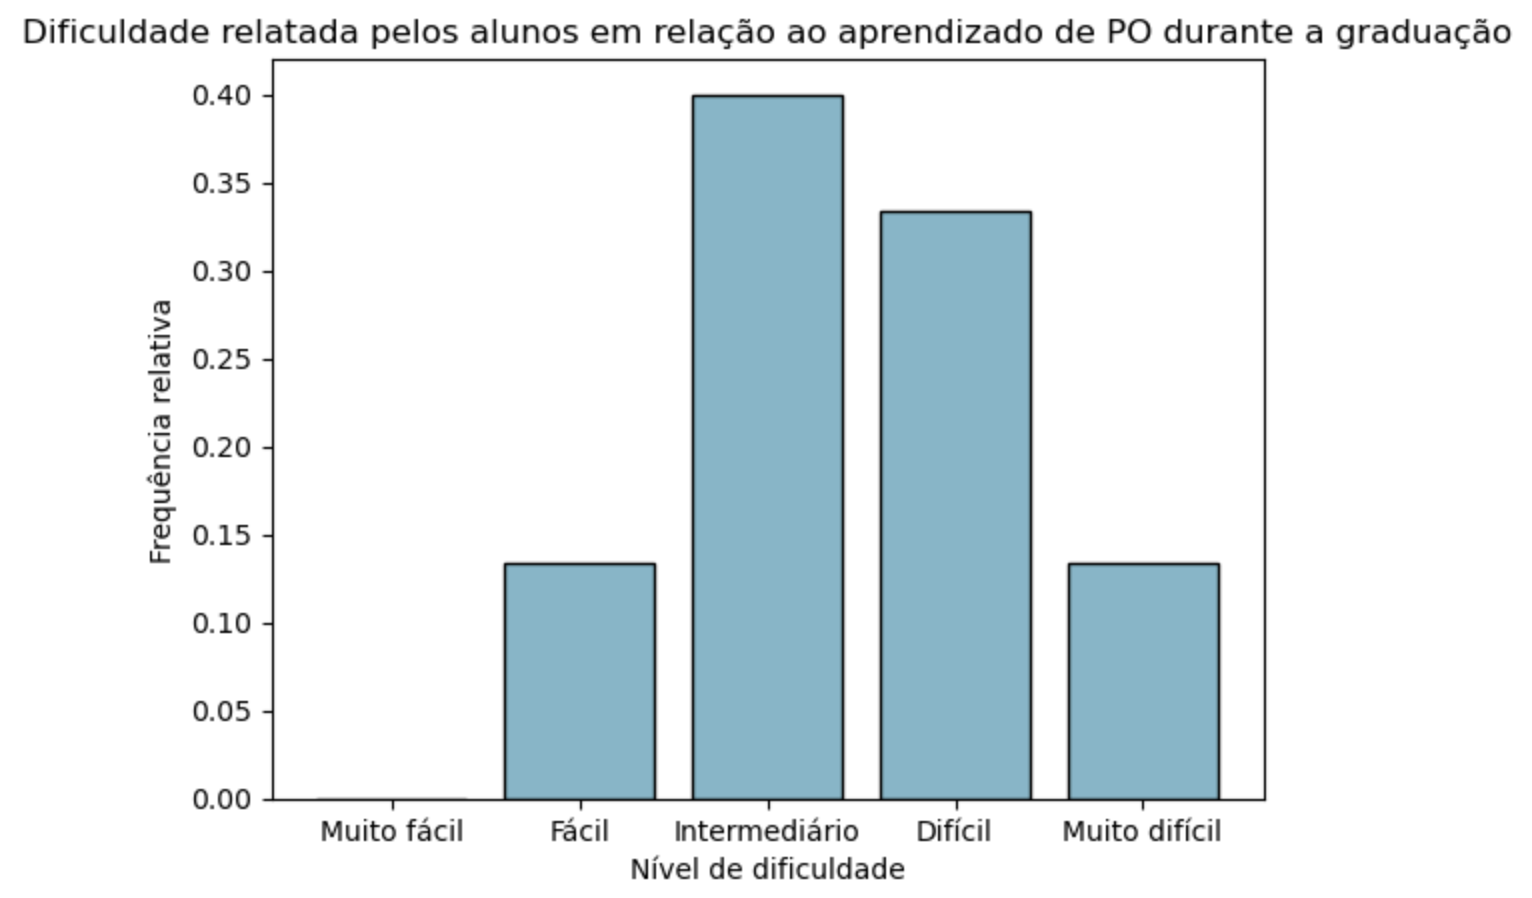
\includegraphics[width=0.6\textwidth]{images/questionary/question-1.png}
\caption{Distribuição de percepções de dificuldade em relação à questão 1.}
\fonte{Fonte: Elaborada pelos autores, 2023}
\label{fig:images/questionary/question-1}
\end{figure}

\item \textbf{Qual ferramenta você prefere utilizar para resolver problemas de Pesquisa Operacional?}

As opções de resposta eram: Software LINDO, planilha eletrônica (ex.: Excel, Google Sheets), solver (ex.: SCIP, Gurobi, GLPK) e linguagem de programação (ex.: Python, R). A Figura \ref{fig:images/questionary/question-2} apresenta a distribuição das respostas em relação a essa questão.

\begin{figure}[H]
\centering
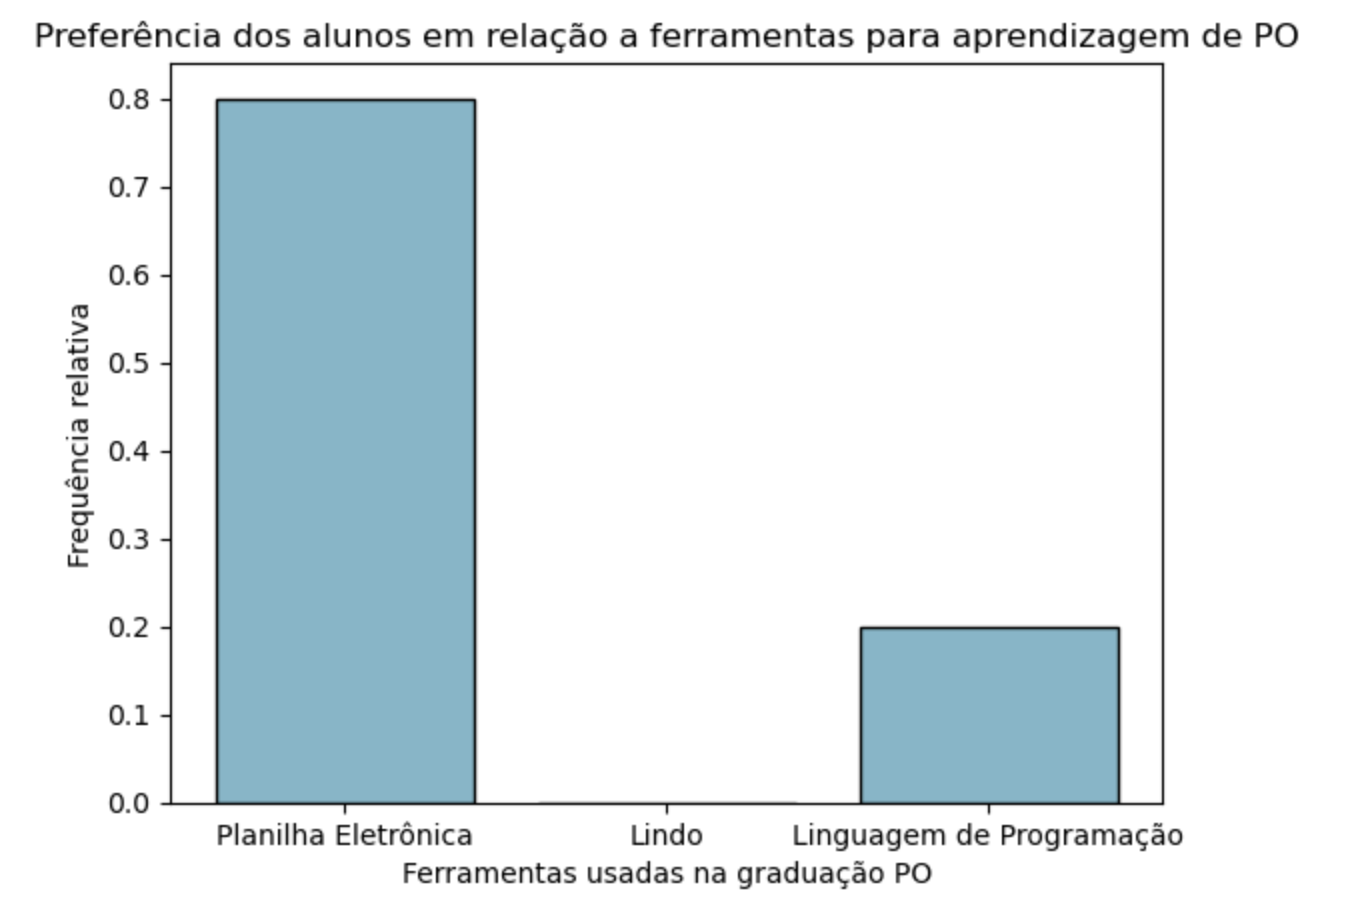
\includegraphics[width=0.6\textwidth]{images/questionary/question-2.png}
\caption{Distribuição de preferências em relação às ferramentas para resolução de problemas de PO em relação à questão 2.}
\fonte{Fonte: Elaborada pelos autores, 2023}
\label{fig:images/questionary/question-2}
\end{figure}

\end{enumerate}

As percepções de dificuldade dos alunos em relação ao aprendizado da disciplina revelaram que cerca de 87\% dos entrevistados a consideram intermediária, difícil ou muito difícil. A resposta "intermediário" foi a mais frequente. Esse resultado sugere que pode haver uma demanda por soluções que ajudem a superar as dificuldades encontradas no processo de aprendizado de PO.

Nesse contexto, a ferramenta proposta neste artigo pode ser uma solução para auxiliar tanto o ensino quanto a aprendizagem de PO, uma vez que ela permite aos alunos visualizar, interagir e explorar diferentes soluções para problemas de otimização, ao mesmo tempo que é capaz de fornecer feedback imediato e intuitivo. Além disso, a integração com planilhas eletrônicas e outras ferramentas de programação pode potencializar a experiência de aprendizagem, possibilitando aos alunos uma abordagem mais prática e contextualizada da disciplina. Com isso, espera-se que a ferramenta possa contribuir para uma melhoria na percepção da dificuldade em relação ao aprendizado de PO.

Com base nos resultados da pesquisa realizada com os alunos do curso de Engenharia de Produção, foi constatado que a maioria dos entrevistados prefere utilizar planilhas eletrônicas (80\%) e linguagens de programação (20\%) como ferramentas para resolver problemas de Pesquisa Operacional (PO). Surpreendentemente, nenhum dos entrevistados mencionou o uso de solvers ou do software LINDO, embora a linguagem formal utilizada nesse software seja semelhante àquela vista nas aulas de PO, ou seja, uma linguagem algébrica mais simples. Essa constatação pode indicar uma possível desconexão entre o conteúdo ensinado em sala de aula e as ferramentas utilizadas pelos alunos na resolução de problemas, o que pode comprometer a qualidade e eficiência do aprendizado.

Esses resultados sugerem que os alunos preferem ferramentas acessíveis e fáceis de usar, como as planilhas eletrônicas, mas podem recorrer a linguagens de programação quando precisam de soluções mais específicas que vão além das funcionalidades das planilhas. A falta de uso de solvers pode indicar uma falta de conhecimento, acesso ou até mesmo barreiras tecnológicas que desencorajem o uso dessas ferramentas durante o estudo da PO na graduação.

Com base nessas observações, é importante considerar o desenvolvimento de uma nova ferramenta para a aprendizagem ativa de PO, que integre a facilidade de uso e a interface visual oferecidas pelas planilhas eletrônicas, enquanto explora a abordagem algébrica utilizada pelo LINDO. Ao combinar essas duas abordagens, a nova ferramenta poderá oferecer uma solução que atenda às necessidades dos alunos e os ajude a aprender a PO de maneira mais eficaz.

\subsection{Delimitação do Escopo da PO}

Para o desenvolvimento de uma aplicação de aprendizagem efetiva, é fundamental definir quais tópicos específicos da Pesquisa Operacional serão abordados. Nesse sentido, o atual artigo definiu a delimitação do escopo para a programação matemática, uma vez que ela engloba técnicas como programação linear, problemas de transporte, problemas de transbordo, problemas de designação e outros. Ao concentrar-se nesses tópicos, os alunos podem aprimorar suas habilidades de modelagem e resolução de problemas matemáticos sujeitos a restrições, preparando-os para enfrentar desafios em áreas como logística, produção e finanças.

A aplicação da aprendizagem ativa, como o Problem-Based Learning, pode ser muito útil nesse contexto. Essa abordagem pedagógica envolve a solução de problemas do mundo real, nos quais os alunos são motivados a investigar e analisar um problema, identificar suas causas, e propor soluções. Ao implementar essa abordagem, os alunos se tornam mais engajados e ativos em seu próprio processo de aprendizagem, desenvolvendo habilidades como a resolução de problemas e a tomada de decisão. Além disso, o uso de exemplos práticos e ferramentas computacionais pode facilitar o aprendizado, tornando-o mais prático e aplicável na resolução de problemas reais.

Construímos a aplicação em torno dessa delimitação da disciplina e estruturando suas funcionalidades baseando-se nas seguintes fases de implementação da Pesquisa Operacional propostas por \citeonline{taha}, a saber: definição do problema, construção do modelo, solução do modelo, validação do modelo e implementação da solução.

Podemos aplicar conceitos da PBL e desenvolver de forma orgânica, durante o uso da ferramenta, uma narrativa que promova imersão do aluno ao problema e desperte sua intuição para os detalhes das restrições, objetivos e possíveis soluções dos problemas. Especialmente para a pesquisa operacional, a contextualização dos problemas torna-se muito importante, conforme afirma \citeonline[p.~3]{wagner}:
\begin{flushright}
    \begin{quote}
    ``A despeito do enorme crescimento na aceitação de modelos de pesquisa operacional, há muito poucas aplicações "padrões". Mesmo em áreas de tomada de decisão onde a relevância de modelos matemáticos tornou-se bem estabelecida, projetar aplicações especiais em companhias específicas requer considerável competência por parte dos pesquisadores. A maior parte dos modelos são formulados sob medida.''
    \end{quote}
\end{flushright}

Assim, a aplicação desenvolvida nesta pesquisa tem como objetivo fornecer uma ferramenta para a modelagem e resolução de problemas de programação matemática, com um enfoque em exemplos e aplicações práticas, como promove a PBL, buscando tornar o aprendizado mais dinâmico e intuitivo para os alunos.

\subsection{Análise Comparativa das Alternativas}

\begin{table}[H]
\centering
\caption{Vantagens e desvantagens de solvers e linguagens de programação para PO}
\label{tab:vantagens-desvantagens}
\begin{tabular}{|p{4cm}|p{4cm}|p{4cm}|}
\hline
\textbf{Ferramentas} & \textbf{Vantagens} & \textbf{Desvantagens} \\ \hline
Planilhas Eletrônicas com Solver interno (Excel, GSheets) & - Acesso fácil e amplo para usuários comuns \par - Interface gráfica amigável \par - Não requer conhecimento em programação & - Limitado a problemas de pequeno e médio porte \par - Pode não encontrar a solução ótima \par - Dificuldade de resolução de problemas complexos \\ \hline
Software LINDO & - Grande capacidade de processamento \par - Interface gráfica amigável \par - Capacidade de lidar com problemas complexos & - Alto custo \par - Requer conhecimento específico para operar e interpretar resultados \\ \hline
Solvers (Gurobi, GLPK, SCIP) & - Alta precisão na resolução de problemas \par - Grande capacidade de processamento \par - APIs disponíveis para diversas linguagens de programação & - Requer conhecimento em programação \par - Pode ser necessário adaptar o modelo para o solver escolhido \\ \hline
Linguagens de Programação (Python, R) & - Flexibilidade para modelagem e resolução de problemas \par - Grande capacidade de processamento \par - Grande comunidade de usuários \par - Open-source & - Requer conhecimento em programação \par - Pode ser necessário implementar funções específicas para o problema em questão \\ \hline
\end{tabular}
\end{table}

A Tabela \ref{tab:vantagens-desvantagens} apresenta ferramentas que podem ser utilizadas no mesmo contexto para resolução de problemas de Programação Matemática/PO. De um modo geral, as planilhas eletrônicas com solver interno são uma boa opção para usuários comuns e problemas de pequeno e médio porte, enquanto solvers como Gurobi, GLPK e SCIP oferecem alta precisão e capacidade de processamento, mas exigem conhecimento em programação. Linguagens de programação como Python e R oferecem flexibilidade e uma grande comunidade de usuários, mas também exigem habilidades em programação. O software LINDO possui uma abordagem de interação simples (um sistema formal bem próximo da álgebra de sala de aula) e é capaz de lidar com problemas complexos, mas requer conhecimento específico para operar, apresenta uma interface gráfica não tão agradável e não tem tanta popularidade quanto as planilhas eletrônicas e linguagens de programação.

Considerando que a proposta da aplicação é uma ferramenta para aprendizado que promove recursos interativos, é necessário escolher e construir suas funcionalidades a partir das vantagens das várias opções apresentadas na tabela. Dessa forma, a proposta pode utilizar uma linguagem de programação como Python ou R, juntamente com pacotes específicos para programação linear. Além disso, a ferramenta pode incluir recursos visuais e interativos, como tabelas e gráficos, que são comuns em planilhas eletrônicas. A interface da aplicação pode ser projetada de forma a ser amigável e intuitiva, buscando trazer as vantagens da interface gráfica do LINDO.

Dessa forma, a proposta da aplicação pode utilizar uma combinação de diferentes ferramentas e recursos para trazer as vantagens de cada uma delas, com o objetivo de criar uma ferramenta para aprendizado de programação matemática que seja flexível, intuitiva e interativa.

\subsection{Ferramentas Tecnológicas}

Nesta etapa do desenvolvimento, detalharemos as ferramentas tecnológicas e a metodologia empregada na construção da aplicação proposta. A criação do aplicativo se baseia em um diagrama conceitual, que servirá como guia para a implementação das funcionalidades da aplicação. Além disso, definimos uma sintaxe de operadores que será utilizada como interface para a criação dos modelos matemáticos, a partir de um sistema formal simplificado.

O diagrama conceitual foi desenvolvido a partir da análise de requisitos do usuário, definindo as funcionalidades necessárias para a aplicação. Com isso, foi possível organizar e estruturar a aplicação de forma intuitiva e coerente com a lógica da Pesquisa Operacional.

A sintaxe dos operadores foi definida com base na análise exposta na Tabela \ref{tab:vantagens-desvantagens}, a qual reflete as necessidades dos usuários em relação às ferramentas de PO. Ela busca ser o mais simples possível, com o objetivo de facilitar o entendimento e a utilização da ferramenta. Dessa forma, os usuários poderão criar modelos matemáticos com mais facilidade e sem a necessidade de possuir conhecimentos avançados em programação.

Para a implementação do aplicativo, foram utilizadas diversas ferramentas tecnológicas, como linguagens de programação, frameworks e bibliotecas. A escolha dessas ferramentas levou em consideração a preferência por recursos open-source, a facilidade de uso, a disponibilidade de documentação e a compatibilidade com as funcionalidades necessárias para a aplicação.

\subsubsection{Python - Linguagem de Programação}

Python é uma linguagem de programação de alto nível, de código aberto, que possui uma sintaxe clara e simples, o que a torna uma das linguagens mais populares para desenvolvimento de software. Possui uma ampla biblioteca padrão que fornece suporte para muitas tarefas comuns, desde a manipulação de strings até a programação em rede. Além disso, a comunidade de desenvolvedores de Python é ativa e crescente, o que significa que há uma grande quantidade de bibliotecas de terceiros disponíveis para quase qualquer tarefa imaginável \cite{python}.

\subsubsection{Streamlit - Framework da Aplicação}

O Streamlit é um framework de código aberto que permite criar rapidamente aplicativos web interativos em Python. Ele oferece uma interface simples e fácil de usar para criar interfaces de usuário (UI) para aplicativos web. Com o Streamlit, é possível criar rapidamente aplicativos interativos de análise de dados, visualização de dados, entre outros, sem precisar se preocupar com a infraestrutura de backend \cite{streamlit}.

\subsubsection{OR-Tools - Pacote com Implementações de Pesquisa Operacional}

O OR-Tools é um pacote de software desenvolvido pelo Google para solução de problemas de otimização. Ele contém uma ampla variedade de solvers de otimização, incluindo programação linear, programação inteira, roteamento, programação de restrições, entre outros. O OR-Tools é escrito em C++, mas possui interfaces para várias linguagens de programação, incluindo Python. Ele é uma ferramenta poderosa para resolver problemas de otimização em uma variedade de campos, como logística, finanças, produção, entre outros \cite{ortools}.
O OR-Tools oferece uma variedade de solvers de otimização, incluindo GLOP, SCIP e Graph.

\subsubsection{Pandas - Biblioteca de Análise de Dados}

O Pandas é uma biblioteca de código aberto para análise de dados em Python. Ele fornece estruturas de dados de alta performance e fáceis de usar, além de ferramentas para manipulação e análise de dados. O Pandas é frequentemente usado em tarefas de ciência de dados, como limpeza, transformação e análise de dados. Ele é capaz de trabalhar com dados de diversos formatos, como arquivos CSV, Excel, SQL, entre outros.

Com o uso do Pandas, é possível carregar dados em memória, realizar operações de filtragem, agregação e transformação, além de outras operações comuns em tarefas de análise de dados. O Pandas também oferece recursos para a visualização de dados, permitindo a criação de gráficos e visualizações de dados de maneira simples e eficiente \cite{pandas}.

\subsection{Desenvolvimento da Aplicação}
\subsubsection{Fluxograma de funcionamento da aplicação}
A interação proposta da aplicação para com o usuário está exemplificada no seguinte diagrama de fluxo da Figura \ref{fig:fluxograma}:

\begin{figure}[H]
\centering
    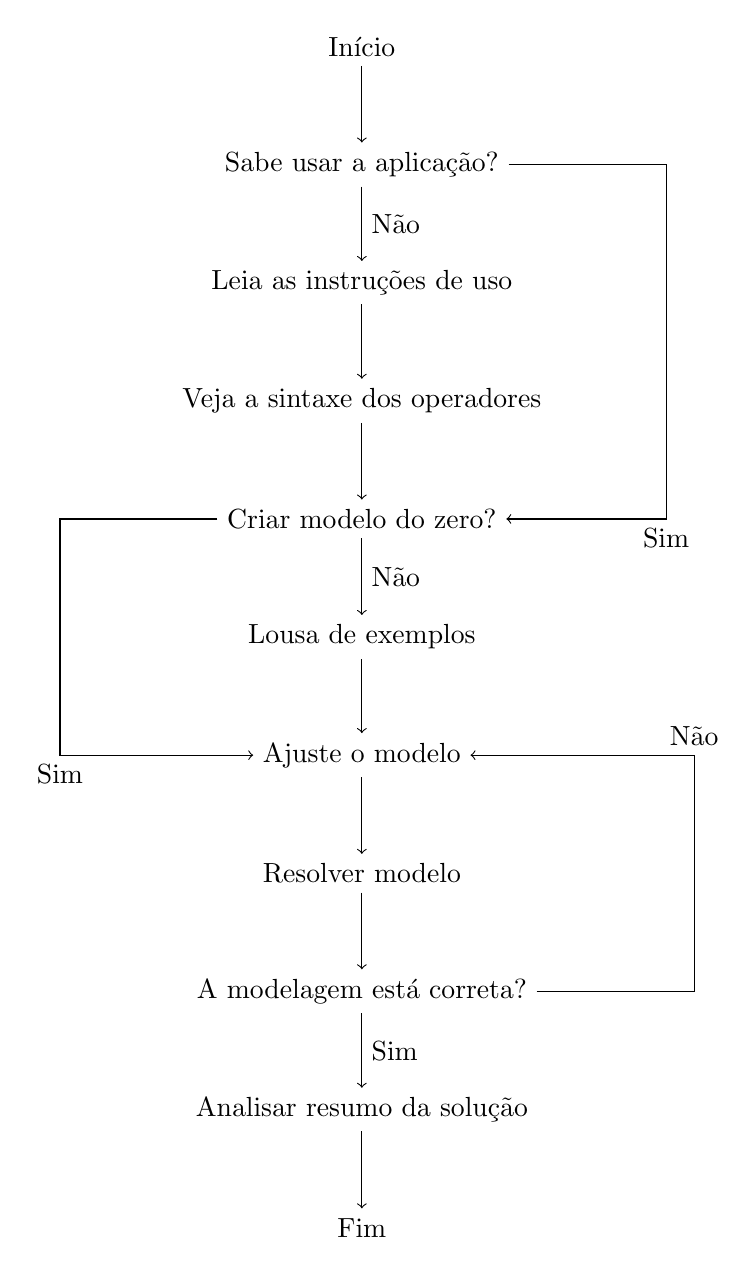
\begin{tikzpicture}[node distance=1.5cm]
        \node (start) {Início};
        \node (pergunta0) [below of=start] {Sabe usar a aplicação?};
        \node (instrucoes) [below of=pergunta0] {Leia as instruções de uso};
        \node (sintaxe) [below of=instrucoes] {Veja a sintaxe dos operadores};
        \node (pergunta1) [below of=sintaxe] {Criar modelo do zero?};
        \node (exemplos) [below of=pergunta1] {Lousa de exemplos};
        \node (ajustar-modelo) [below of=exemplos] {Ajuste o modelo};
        \node (resolver) [below of=ajustar-modelo] {Resolver modelo};
        \node (pergunta2) [below of=resolver] {A modelagem está correta?};
        \node (analisar) [below of=pergunta2] {Analisar resumo da solução};
        \node (fim) [below of=analisar] {Fim};

        \draw [->] (start) -- (pergunta0);
        \draw [->] (pergunta0) -- node[right]{Não} (instrucoes);
        \draw [->] (pergunta0.east) -- +(2,0) |- node[below]{Sim} (pergunta1);
        \draw [->] (instrucoes) -- (sintaxe);
        \draw [->] (sintaxe) -- (pergunta1);
        \draw [->] (pergunta1) -- node[right]{Não} (exemplos);
        \draw [->] (pergunta1.west) -- +(-2,0) |- node[below]{Sim} (ajustar-modelo);
        \draw [->] (exemplos) -- (ajustar-modelo);
        \draw [->] (ajustar-modelo) -- (resolver);
        \draw [->] (resolver) -- (pergunta2);
        \draw [->] (pergunta2.east) -- +(2,0) |- node[above]{Não} (ajustar-modelo);
        \draw [->] (pergunta2) -- node[right]{Sim} (analisar);
        \draw [->] (analisar) -- (fim);
    \end{tikzpicture}
    \caption{Fluxograma da jornada do usuário no SolvedOR.}
    \fonte{Fonte: Elaborada pelos autores, 2023}
    \label{fig:fluxograma}
\end{figure}

Um aspecto importante a ser destacado no diagrama proposto é a ênfase na iteração do processo de modelagem. Espera-se que erros ocorram ao longo do caminho, e a ideia é que estes erros sejam identificados e corrigidos à medida que se desenvolve, testa e avalia o que foi criado. Dessa forma, o processo de modelagem se torna um ciclo contínuo de aprimoramento, no qual as etapas são revisadas e ajustadas para a obtenção de um modelo cada vez mais preciso e eficiente.

\subsubsection{Sintaxe dos Operadores}
A lousa é a interface de interação para que os alunos possam construir seus modelos e registrar comentários. Para que seja funcional e dinâmica, foi criada uma sintaxe formal simples utilizando a biblioteca re do Python que fornece funcionalidades Regex que permite o trabalho com padrões de caracteres. Dessa forma, foi possível utilizar uma linguagem algébrica, similar àquela utilizada em salas de aula, para definir os modelos de programação matemática. A sintaxe proposta utiliza marcadores que antecedem as definições dos modelos, permitindo que a aplicação capture essas definições e gere um modelo que possa ser resolvido.

Um modelo de programação matemática simples estudado nos cursos de Pesquisa Operacional na graduação contém a função objetivo, as restrições e o tipo de problema (linear, inteiro ou misto).

Para definir o tipo de problema, o usuário pode utilizar os marcadores 'problema' ou 'p' seguidos de dois pontos (:), conforme o exemplo a seguir:

\begin{center}
\texttt{p: linear}
\end{center}

Para definir a função objetivo do modelo, o usuário deve utilizar os marcadores 'max' ou 'min' seguidos de dois pontos (:), seguidos da função objetivo no formato '2x1 + 3x2 + 4x3 + 5x4', conforme o exemplo a seguir:

\begin{center}
\texttt{min: 2x1 + 3x2 + 4x3 + 5x4}
\end{center}

Para definir as restrições às quais o modelo deve estar sujeito, o usuário deve utilizar os marcadores 'restricao' ou 'r' seguidos de dois pontos (:), conforme o exemplo a seguir:

\begin{center}
\texttt{r: 2x1 + 3x2 + 4x3 + 5x4 <= 10}
\end{center}

O operador de comparação (<=, =, >=) e o termo do lado direito da restrição também devem ser especificados. Vale ressaltar que o operador utilizado para representar a multiplicação é o asterisco (*), ao invés do sinal de multiplicação (x) utilizado no exemplo acima.

Para definir o arredondamento dos valores no modelo, o usuário pode utilizar os marcadores "arred", "arredondamento" ou "round", seguidos de ":" e o número de casas decimais desejado. Caso o arredondamento não seja definido, a aplicação considerará o valor padrão de 5 casas decimais, conforme o seguinte exemplo:

\begin{center}
\texttt{arred: 2}
\end{center}

Exemplo de um modelo matemático que poderia ser visto em sala de aula:

\begin{equation*}
\begin{aligned}
\max \quad & 8x_1 + 10x_2 \\
\text{s.a.} \quad & 0.5x_1 + 0.5x_2 \leq 150 \\
& 0.6x_1 + 0.4x_2 \leq 145 \\
& 30 \leq x_1 \leq 150 \\
& 40 \leq x_2 \leq 200 \\
& x_1, x_2 \geq 0
\end{aligned}
\end{equation*}

Exemplo completo do mesmo modelo utilizando a sintaxe proposta:

\begin{center}
\begin{varwidth}{\linewidth}
\begin{verbatim}
problema: linear

max: 8x1 + 10x2

restricao: 0.5x1 + 0.5x2 <= 150
restricao: 0.6x1 + 0.4x2 <= 145

restricao: 30 <= x1 <= 150
restricao: 40 <= x2 <= 200

restricao: x1 >= 0
restricao: x2 >= 0

arredondamento: 3
\end{verbatim}
\end{varwidth}
\end{center}

O modelo acima representa um problema de programação linear que busca maximizar a função objetivo $8x_1 + 10x_2$ sujeito a um conjunto de restrições lineares. As restrições impõem limites para as variáveis $x_1$ e $x_2$ e garantem que a solução encontrada satisfaça as demandas do problema em questão.

É importante notar que a sintaxe proposta busca ser o mais simples possível, visando facilitar o entendimento e a utilização da ferramenta pelos usuários.

\subsubsection{Instruções de uso e guia do usuário}

\begin{figure}[H]
\centering
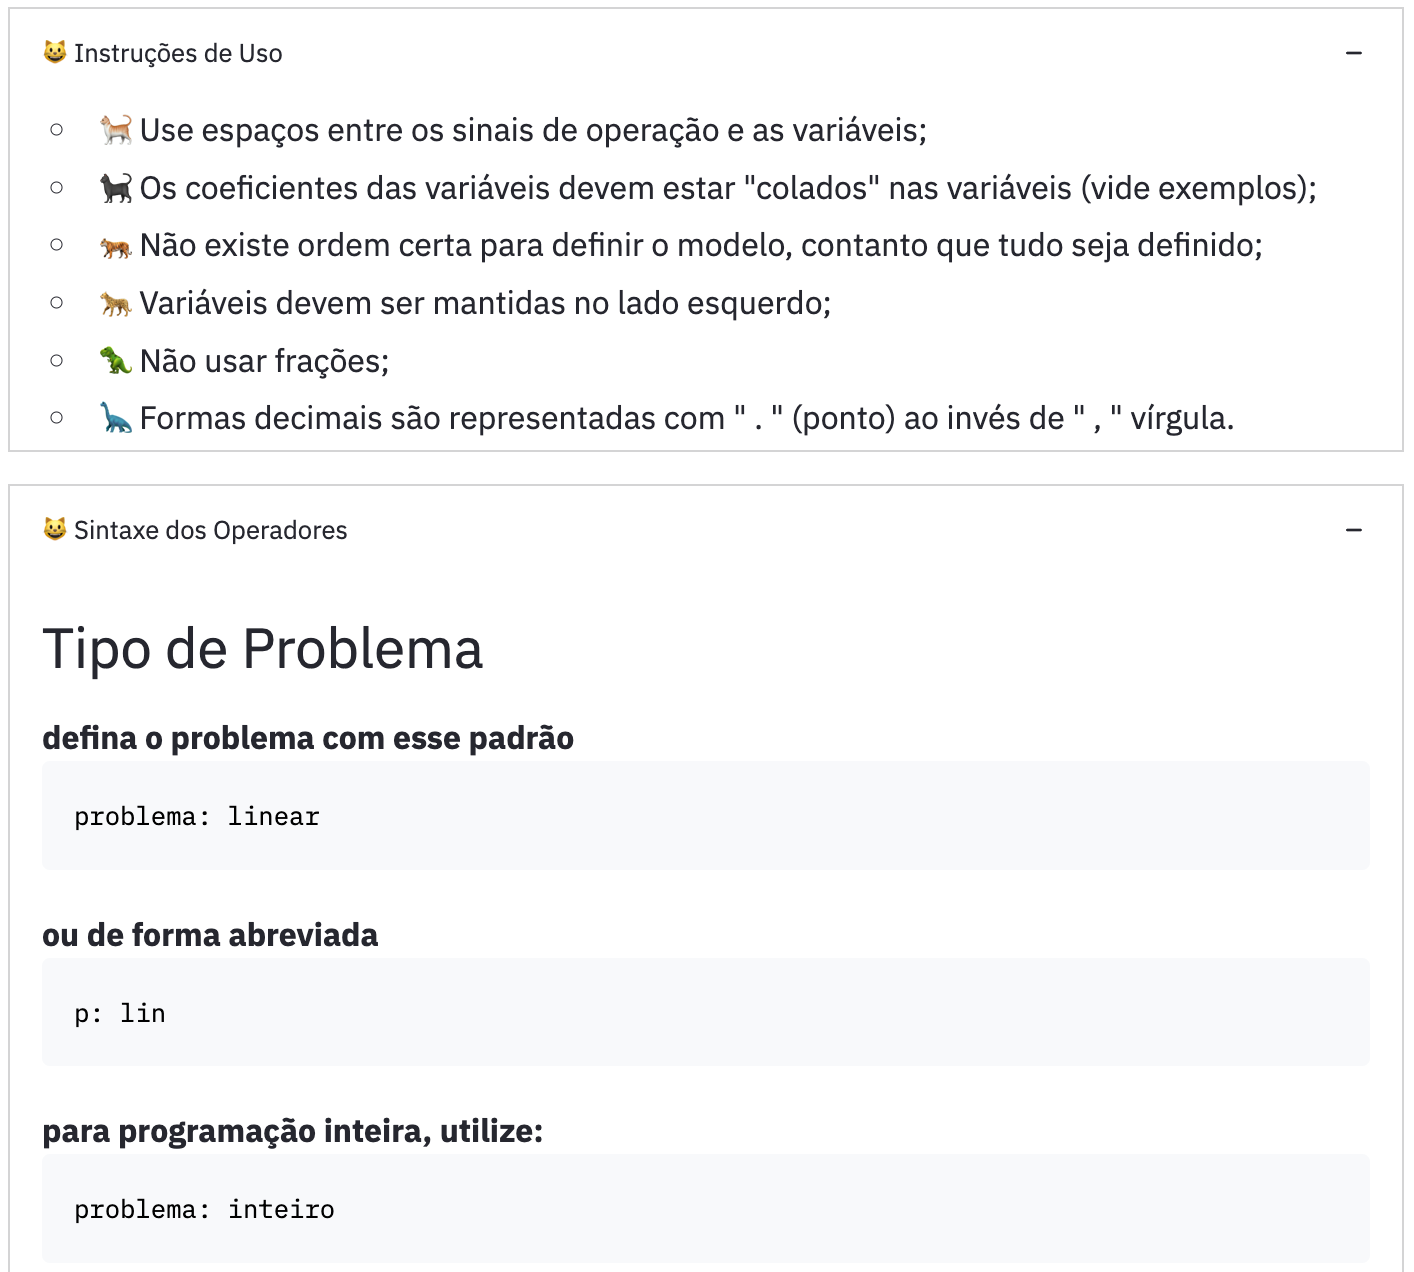
\includegraphics[width=0.6\textwidth]{images/app/instructions-and-guide.png}
\caption{Contêiner contendo as instruções de uso e parte da sintaxe dos operadores.}
\fonte{Fonte: Elaborada pelos autores, 2023}
\label{fig:images/app/instructions-and-guide}
\end{figure}

A seção de instruções ilustrada pela Figura \ref{fig:images/app/instructions-and-guide} apresenta um contêiner que contêm a comunicação de boas práticas e padrões que guiam a criação dos modelos na aplicação. Na parte inferior da mesma imagem, podemos ver parte do guia que dá instruções a respeito das sintaxes que o usuário deve utilizar para definir função objetivo, restrição e outros detalhes da modelagem.

\subsubsection{Lousas de exemplo e solução}
A lousa de exemplos foi criada para fornecer um espaço onde professores possam disponibilizar uma lista de modelos prontos para seus alunos. A intenção é que esses exemplos possam ajudar a guiar os alunos na resolução de problemas inéditos relacionados aos temas que estão sendo ensinados, conforme ilustrado na Figura \ref{fig:images/app/example-board-list}. Nessa área, é possível adicionar um enunciado escrito ou uma imagem para fornecer contexto e promover uma melhor imersão dos alunos durante o estudo e resolução de problemas.

\begin{figure}[H]
\centering
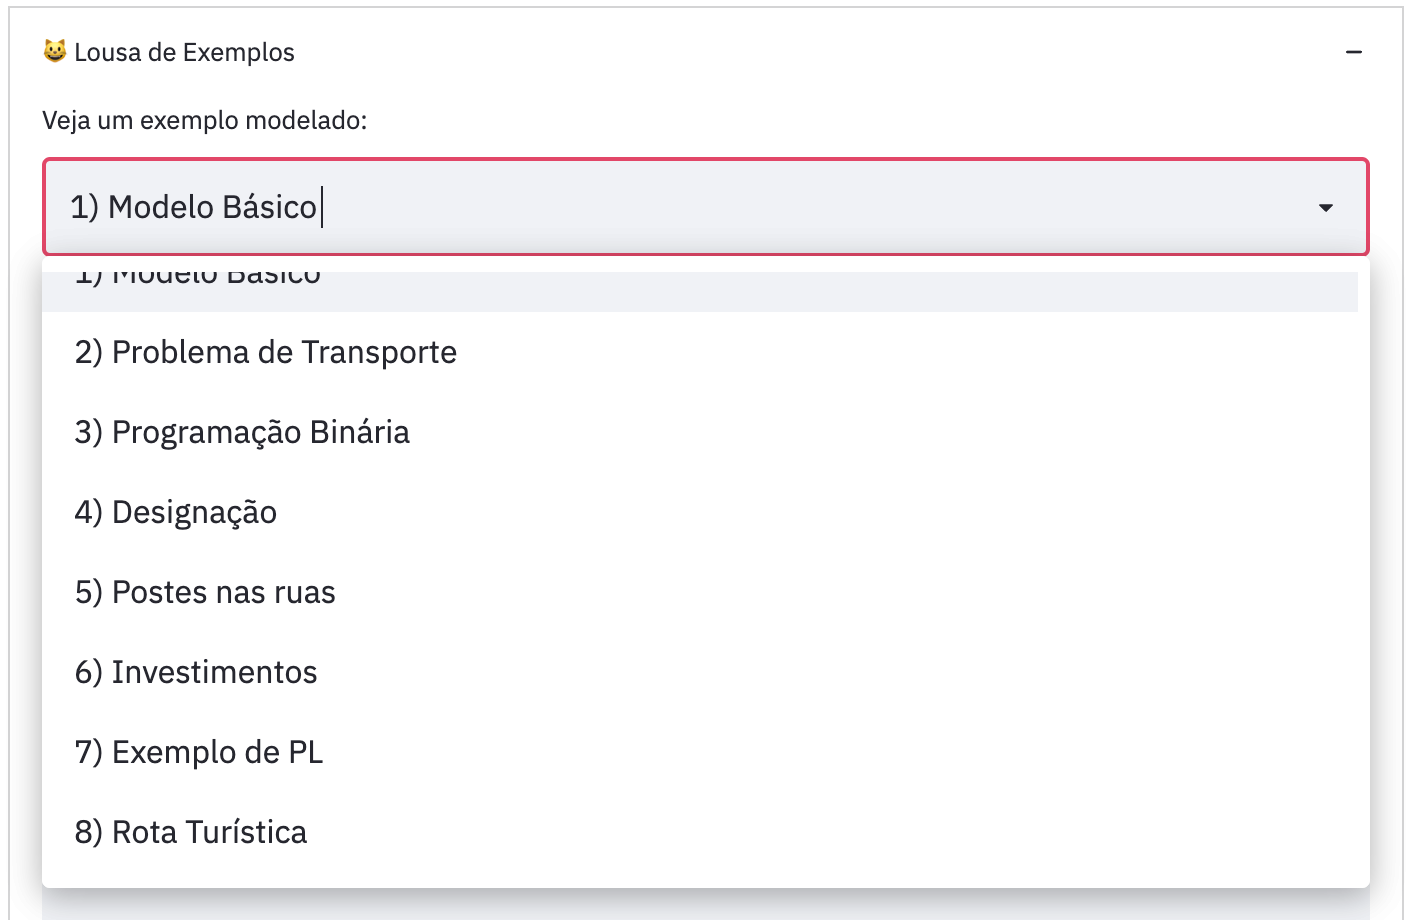
\includegraphics[width=0.6\textwidth]{images/app/example-board-list.png}
\caption{Contêiner da lousa de exemplos com uma lista suspensa dos modelos prontos disponíveis.}
\fonte{Fonte: Elaborada pelos autores, 2023}
\label{fig:images/app/example-board-list}
\end{figure}

A lousa de soluções é o espaço dedicado à construção da modelagem. É semelhante à lousa de exemplos, porém, nesse espaço, as soluções são efetivamente construídas e resolvidas. A diferença crucial é que a lousa de soluções é o local onde os alunos têm a oportunidade de aplicar os conhecimentos adquiridos para resolver problemas inéditos e desenvolver suas habilidades em PO. Desde que as regras de sintaxe dos operadores sejam obedecidas, é possível adicionar comentários e fazer anotações de maneira livre.

\subsubsection{Resumo da solução}

Apresenta os resultados obtidos a partir do preenchimento do modelo na lousa de soluções, atualizando a seção de resumo com os dados do modelo atual. A Figura \ref{fig:images/app/solution-summary} exemplifica essa atualização, exibindo os detalhes da solução presente na lousa.

\begin{figure}[H]
\centering
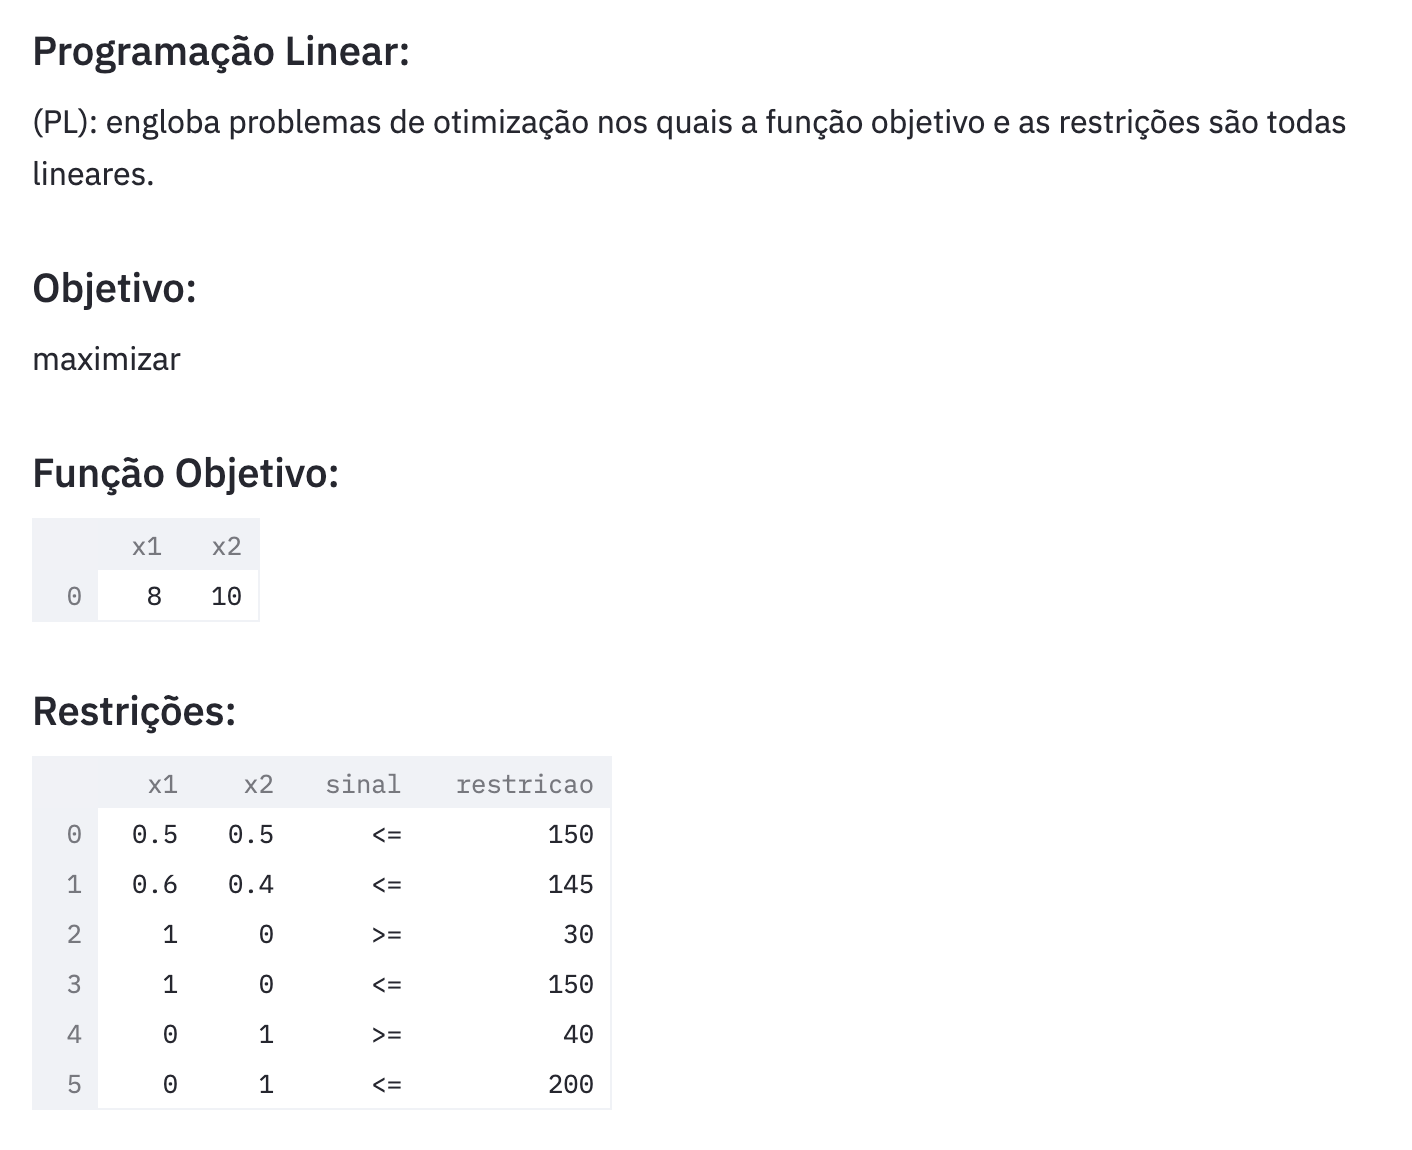
\includegraphics[width=0.6\textwidth]{images/app/solution-summary.png}
\caption{Seção de resumo com os detalhes da solução atual presente na lousa de soluções.}
\fonte{Fonte: Elaborada pelos autores, 2023}
\label{fig:images/app/solution-summary}
\end{figure}

Para visualizar a solução do modelo descrito, é possível apertar o botão "Resolver", o que irá gerar uma mensagem informando se o modelo possui solução ótima, factível, entre outras possibilidades. Na Figura \ref{fig:images/app/results}, é possível visualizar o resultado otimizado da função objetivo e os valores correspondentes das variáveis do problema. Além disso, é apresentada a duração da execução do algoritmo de otimização, bem como o número de iterações necessárias para atingir o resultado (que pode variar de acordo com o algoritmo utilizado pelo solver).

\begin{figure}[H]
\centering
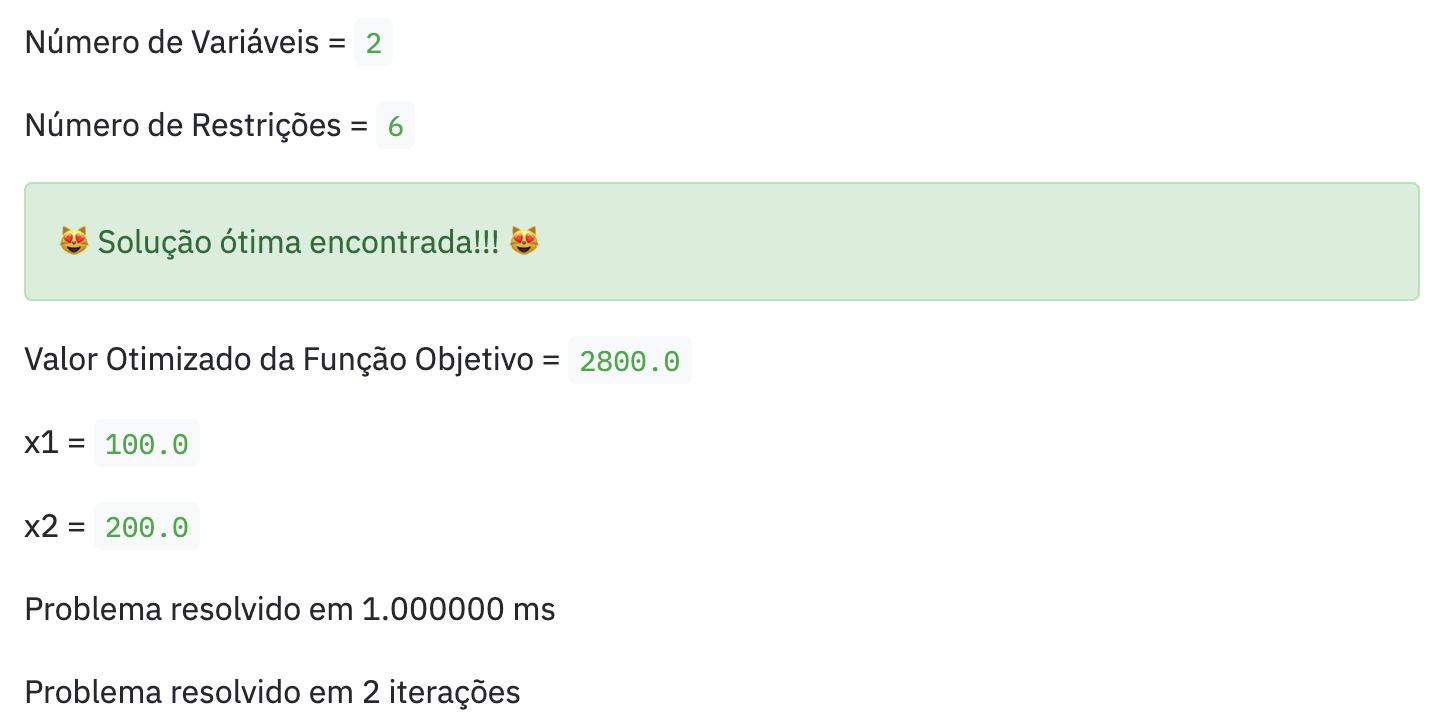
\includegraphics[width=0.6\textwidth]{images/app/results.png}
\caption{Resultado gerado pela solução do modelo através de um solver do OR-Tools.}
\fonte{Fonte: Elaborada pelos autores, 2023}
\label{fig:images/app/results}
\end{figure}

Uma abordagem interessante para facilitar a compreensão e análise dos resultados em modelos matemáticos e de otimização é a utilização de figuras dinâmicas. Essas figuras permitem a visualização gráfica das restrições e função objetivo, e a geração de gráficos interativos, quando aplicável. De acordo com \citeonline{amado}, essa abordagem potencializa o raciocínio lógico-dedutivo, uma vez que os resultados invariantes são facilmente perceptíveis conforme o aluno explora os gráficos interativos. Com essa metodologia, os alunos podem assimilar melhor a problemática através de sua interpretação geométrica.

A Figura \ref{fig:images/app/plot} exemplifica um desses gráficos, que apresenta as regiões delimitadas pelas restrições que restringem os valores das variáveis do problema, as curvas geradas pelas restrições de inequação e destaca o ponto que otimiza a função objetivo.

\begin{figure}[H]
\centering
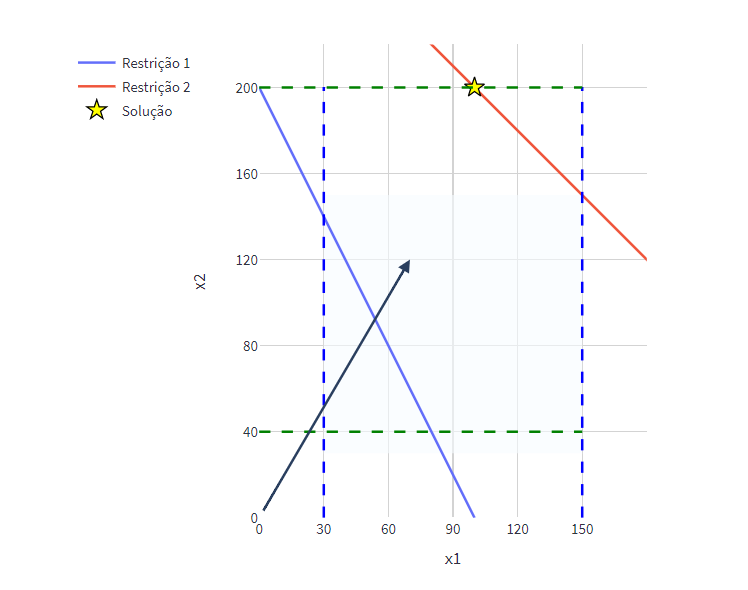
\includegraphics[width=0.6\textwidth]{images/app/plot.png}
\caption{Gráfico gerado a partir do modelo criado destacando os traços das restrições e a solução encontrada.}
\fonte{Fonte: Elaborada pelos autores, 2023}
\label{fig:images/app/plot}
\end{figure}

O gradiente destacado na Figura \ref{fig:images/app/plot} indica a direção de crescimento da função objetivo, ou seja, a direção em que o valor da função cresce mais rapidamente. A compreensão do gradiente é fundamental para o entendimento da otimização em problemas de programação matemática e pode ser explicado de forma mais detalhada aos alunos.

Por fim, cabe ressaltar que o formato tabular apresentado na seção de resumo é semelhante às planilhas eletrônicas, o que torna mais familiar e acessível aos estudantes.

\subsection{Avaliação do software pelos usuários}

O software foi disponibilizado para usuários que já o utilizaram ou estavam utilizando-o e foi solicitado que eles fornecessem feedback em relação aos seguintes critérios:

\begin{itemize}
\item Funcionalidade: Durante o teste, foi observado que a maioria dos usuários conseguiu realizar as tarefas facilmente e não tiveram dificuldade em entender as instruções. No entanto, foram identificados problemas em algumas das funcionalidades da sintaxe (impossibilidade de criar variáveis com nomes mais descritivos do que variantes de 'x') e necessidade de espaços exatos entre as variáveis e sinais que foram adicionadas ao backlog de mudanças.
\item Design: Após o uso do software, a pesquisa de satisfação mostrou que a maioria dos usuários avaliou positivamente a experiência em relação ao design, destacando a simplicidade e a clareza da interface. No entanto, alguns usuários sugeriram melhorias na organização dos elementos e na paleta de cores utilizada. Isto também foi incluído no backlog e alterado.
\item Performance: Os usuários avaliaram positivamente a performance do software, destacando a rapidez na execução de tarefas e na apresentação dos resultados. Até mesmo usuários em computadores com configurações mais modestas foram capazes de utilizar a aplicação sem ocorrências de travamentos.
\item Confiabilidade: Foi identificado um consenso entre os usuários em relação à confiabilidade do software, destacando a consistência dos resultados gerados e a ausência de erros ou falhas durante o uso. Foi sugerido que os usuários resolvessem seus problemas na ferramenta proposta e com as alternativas para efeito de validação, o que não resultou em inconsistências.  Utilizar uma biblioteca com métodos de PO desenvolvida pelo Google, que é o caso da OR-Tools, promove essa confiabilidade. A disponibilização de arredondamento customizável foi um ponto positivo destacado pelos usuários.
\end{itemize}

Além dessa iteração e correção de funcionalidades que foi feita durante os primeiros testes com os usuários, houve uma disponibilização de um formulário com 2 perguntas fechadas que tem como objetivo avaliar o quão bem a solução proposta e desenvolvida atingia os objetivos determinados no início deste estudo.
O formulário foi disponibilizado para alunos voluntários que utilizaram a aplicação, sendo alunos que já cursaram ou que estavam cursando a matéria de Pesquisa Operacional do curso de engenharia de produção da UFAM.

A pesquisa consistiu em um questionário com duas perguntas fechadas. A primeira pergunta indagava se os usuários substituiriam sua ferramenta preferida pela aplicação. Os resultados mostraram que 40\% dos entrevistados afirmaram que sim, enquanto outros 40\% disseram que talvez, conforme a Figura  \ref{fig:images/questionary/feedback-1}. A existência de uma parcela igualmente significativa de usuários que não substituiria sua ferramenta preferida sugere a necessidade de melhorias e ajustes na solução desenvolvida, a fim de torná-la mais competitiva e atraente em relação a outras ferramentas disponíveis no mercado. Além disso, é importante destacar que a aplicação possui um escopo bem mais reduzido em comparação às alternativas já existentes, o que pode limitar sua utilização em alguns casos.

\begin{figure}[H]
\centering
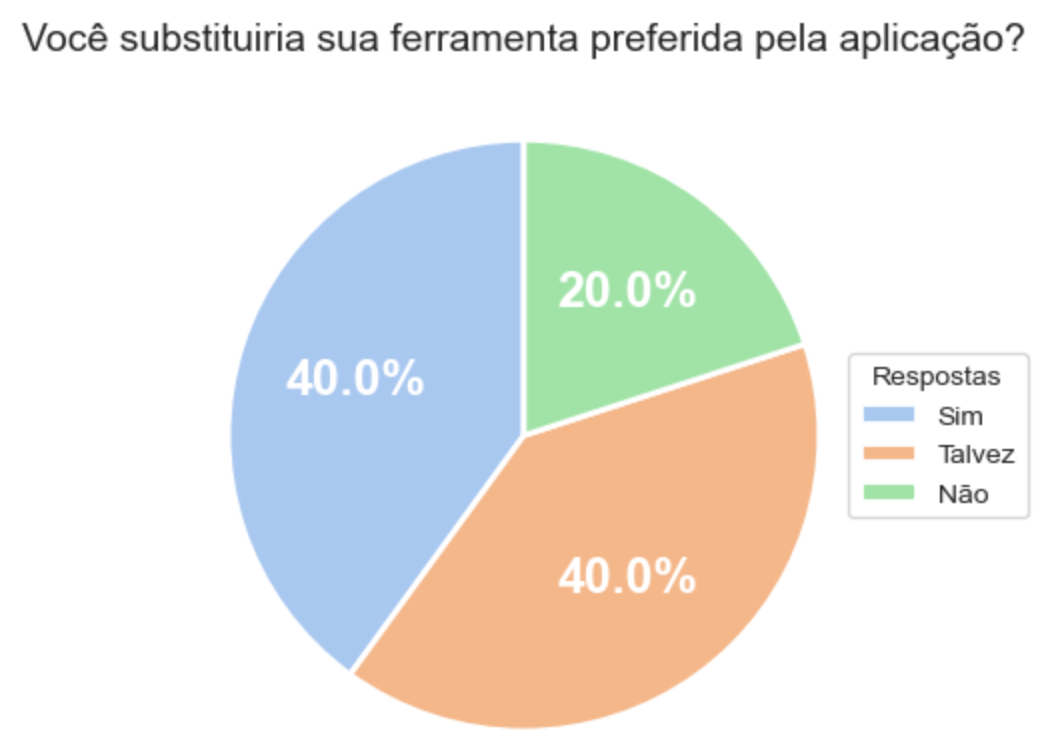
\includegraphics[width=0.6\textwidth]{images/questionary/feedback-1.png}
\caption{Percentual de usuários que substituiriam sua ferramenta preferida pelo SolvedOR.}
\fonte{Fonte: Elaborada pelos autores, 2023}
\label{fig:images/questionary/feedback-1}
\end{figure}

A segunda pergunta da pesquisa indagava qual o grau de dificuldade para construir um modelo de programação matemática na aplicação. Conforme ilustrado na Figura \ref{fig:images/questionary/feedback-2}, os resultados mostraram que 80\% dos entrevistados classificaram como 'Fácil' ou 'Muito Fácil' a construção de um modelo na aplicação, o que indica que a solução desenvolvida atingiu um bom nível de usabilidade e acessibilidade.

\begin{figure}[H]
\centering
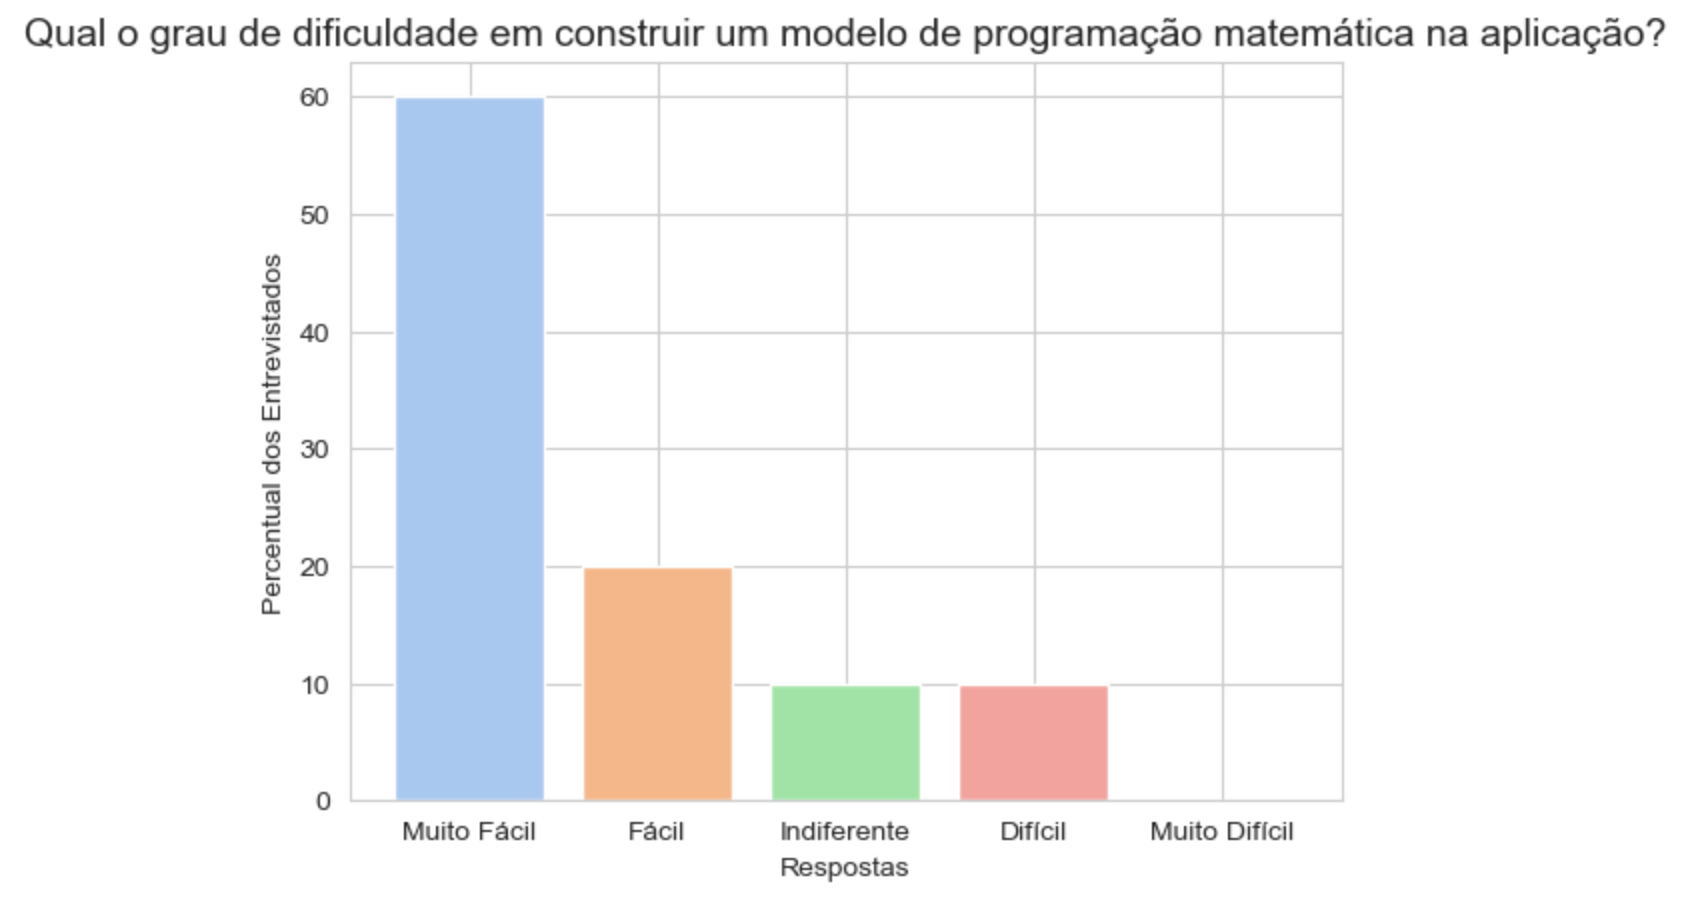
\includegraphics[width=0.8\textwidth]{images/questionary/feedback-2.png}
\caption{Grau de dificuldade para construção de modelo de programação matemática na aplicação.}
\fonte{Fonte: Elaborada pelos autores, 2023}
\label{fig:images/questionary/feedback-2}
\end{figure}

Os resultados desta etapa reforçam a importância de uma avaliação constante do usuário na concepção e desenvolvimento de soluções de programação matemática, a fim de garantir que as soluções desenvolvidas atendam às necessidades e expectativas dos usuários.

Uma possibilidade futura seria a aplicação de uma análise hierárquica à medida que o aplicativo ganha mais adesão e maturidade. Dessa forma, seria possível coletar feedbacks mais consolidados sobre a ferramenta em comparação às suas alternativas com fins didáticos. Isso permitiria uma avaliação mais precisa do desempenho e das funcionalidades do aplicativo em relação aos seus concorrentes, e ajudaria a identificar áreas que precisam ser aprimoradas.

\section{CONCLUSÃO}

A aplicação desenvolvida utilizando princípios de aprendizagem ativa foi capaz de envolver os alunos em um processo de ensino-aprendizagem mais interativo. Ao permitir que os alunos aplicassem os conceitos de forma prática e personalizada, a ferramenta aumentou a motivação e o engajamento dos alunos, o que, por sua vez, pode melhorar a compreensão e retenção dos conceitos.

Embora a ferramenta desenvolvida tenha sido bem recebida pelos alunos, é importante ressaltar que a sua eficácia depende da adoção e do engajamento dos professores. Como não houve um período de experimentação da ferramenta com professores em sala de aula, a aplicação dos conceitos de Aprendizagem Ativa ficou limitada às perspectivas dos alunos, e essa ausência de feedbacks estruturados do corpo docente pode ser considerada uma limitação. Além disso, é importante que a aplicação seja utilizada de forma complementar, não substituindo o papel do professor na sala de aula.

De maneira geral, o desenvolvimento desta aplicação para auxiliar o aprendizado da pesquisa operacional, utilizando conceitos de aprendizagem ativa, proporcionou uma abordagem inovadora e eficaz que pode ser adaptada para outras disciplinas técnicas ou quantitativas. Embora tenha sido focado nos alunos de Engenharia de Produção, a simplicidade alcançada permite que seja aplicado a outras turmas, mesmo que não tenham tanta naturalidade com a linguagem matemática utilizada.

Conclui-se que foi possível capturar as percepções dos estudantes e traduzir esse entendimento em uma ferramenta educacional que apresentasse funcionalidades que anteriormente estavam espalhadas entre as alternativas existentes. Por fim, é essencial que este trabalho possa inspirar a exploração de outras possibilidades tecnológicas que potencializem a educação e aprendizagem. A tecnologia pode oferecer muitas oportunidades para inovar e transformar a forma como as disciplinas são ensinadas e aprendidas. Com isso, pode-se oferecer aos alunos uma experiência mais envolvente e interativa, o que pode levar a uma melhor compreensão e retenção dos conceitos.

\renewcommand{\refname}{REFERÊNCIAS}
\bibliographystyle{abntex2-alf}
\bibliography{references}

\end{document}
